%
% ---- Technologies
%

\section{Technologies}
\begin{shaded}
Some notes about the choice of technologies... two aspects, right-sizing and measuring/routing demand and throughput, have chosen the latter, refer to some of the work on the former?
\end{shaded}

%
% ---- Middleware
%

\subsection{Middleware}

Good choice of middleware in a system will help ensure that its components are connected, but loosely coupled.  If, for example, a web server is blocked waiting for a response from a worker application carrying out a more expensive operation, then the throughput of the web server will be limited to that of the worker application.  Also, failure of one of the processes in a distributed system may cause failure of the system as a whole.

\paragraph{Synchronous vs Asynchronous Middleware.}
With synchronous middleware such as Remote Procedure Call (RPC), the calling process is blocked until the called service completes and returns control to the caller.  The system components are tightly coupled.  This is undesirable for our ticketing application.

Distributed systems using some form of asynchronous middleware do not block when calling a remote service.  Control is immediately passed back to the caller, and a response may be returned eventually, with the caller polling the remote service for the response, or the remote process calling a method in the caller to send the response.

The ``return'' operation use case does not require a direct response from the system.  As long as the customer can rely on eventual guaranteed delivery of the return request, (and that the cost of their ticket will be refunded) then they do not need to wait for a direct response to their return.

\subsubsection{Message-Oriented Middleware (MOM).}  MOM is a form of Asynchronous Middleware, commonly provided by Larger Cloud service providers such as Amazon Web Services and Microsoft Azure.  These brokered message services provide an intermediate layer between senders and receivers, decoupling their communication.  Message delivery may take minutes rather than milliseconds, but the service providers do provide configurable delivery guarantees \cite{RN65}.

There are two main messaging models, both of which are offered by Microsoft Azure Service Bus \cite{RN1072} for example.

\paragraph{Point-to-Point Queues.} Azure Queues are a point-to-point service implementing First In, First Out (FIFO) message delivery. Many processes may send messages to a queue, and each message is received by one consumer - though it may be one of several consumers competing for messages from this queue.  This competing consumer pattern offers a means of balancing load from the Web servers between the Worker Applications in the ticketing use case.

\paragraph{Publish/subscribe.}  Publish/subscribe (in Azure, topics and subscriptions) are a properly one-to-many or many-to-many communication mechanism.  Any single producer may send one message to a topic, and then all consumers that subscribe to that topic receive a copy of the same message.

%
% ---- Microservices
%

\subsection{Microservices}

Microservice architecture is an approach to structuring applications as suites of small services, defined by business capability verticals rather than technological layers \cite{RN1069} \cite{RN1070}.  Each of the use case requirements - search for tickets, book tickets, return tickets - might typically be microservices with their own worker applications and data nodes.  Ticket data would be denormalised across the data nodes and made eventually consistent via a backplane messaging service \cite{RN1071}.  This would certainly isolate the demand for search, book and return from each other - returning tickets would not be blocked by a system where booking tickets was overloaded.  In the ticketing use case however, there is skewed demand for Athletics tickets.  In a real-world system the booking microservice might be further broken down to a lower level of granularity to deal with this, i.e. a separate microservice for booking each ticket type.

\begin{figure}
\caption{Microservices}
\centering
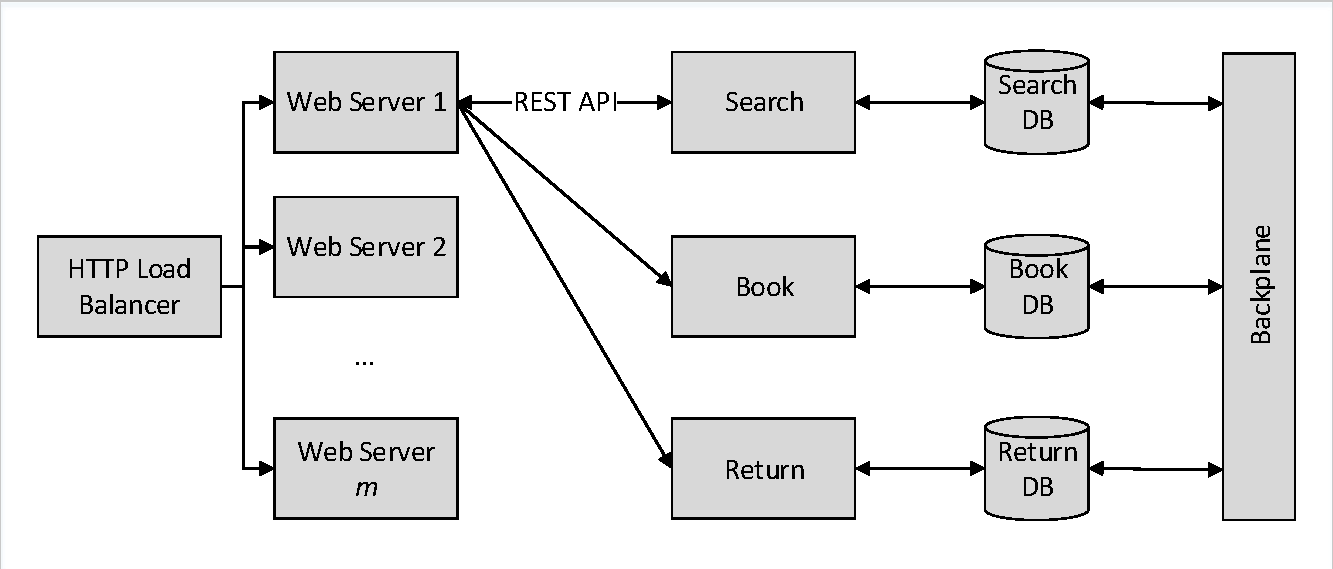
\includegraphics[trim = 5 5 5 5, clip, width=\textwidth]{img/microservices}
\end{figure}

%
% ---- Distributed databases
%

\subsection{Distributed databases}
Modern databases both SQL and NoSQL are designed to scale both data and the load of operations accessing that data over many servers that do not share disk or RAM, so-called ``shared nothing'' architecture \cite{RN67}.  We may partition data {\itshape vertically}, dividing tables into groups of columns that may be placed on different data nodes; or {\itshape horizontally}, where the split is by row \cite{RN68}. 

In the use case, the quantity of data does not approach the levels of ``Big Data'' applications.  Partitioning is proposed instead as a means of scaling the demand for that data.  The ticketing system will not require a large number of columns and the three operations outlined do not have significantly different column requirements, therefore horizontal partitioning is most relevant.  The partition key of a Ticket table may be the Ticket Type, the Date, or the seat Row.  Demand for tickets is likely to vary by each of these attributes.  An alternative partitioning strategy would be to on denormalised tables supporting the query, book and return operations.  The load on each data node would follow the demand for the data types and operations placed there.

The scalability of distributed databases usually comes at the price of a relaxed consistency model - so-called BASE (Basically Available, Soft state, Eventually Consistent) rather than ACID (Atomic, Consistent, Isolated, Durable) transactions.  In the ticketing system, eventual consistency is clearly sufficient for the return ticket scenario - returned tickets do not have to be made immediately available for booking.  Individual ticket bookings must exist on only one partition to prevent the same ticket being booked more than once.  Eventual consistency between search and book operations requires the customer to tolerate the concept of ``reservation'' of a ticket for a short period until a booking can be confirmed \cite{RN1071}\cite{RN67}.

\begin{shaded}
Discuss Cassandra replication model, and refer to other distributed databases using it

Another issue to be aware of is {\itshape replication}.   Most distributed databases offer replication of data from one partition to another for availability.  In the use case, if a data node is overloaded by demand, the system may failover to a copy of the data on another data node, but this will just transfer the demand elsewhere.  If this is also the primary data node of an otherwise low demand data type, then it may be overwhelmed in turn.
\end{shaded}

\begin{figure}
\caption{Distributed database, without and with replication}
\centering
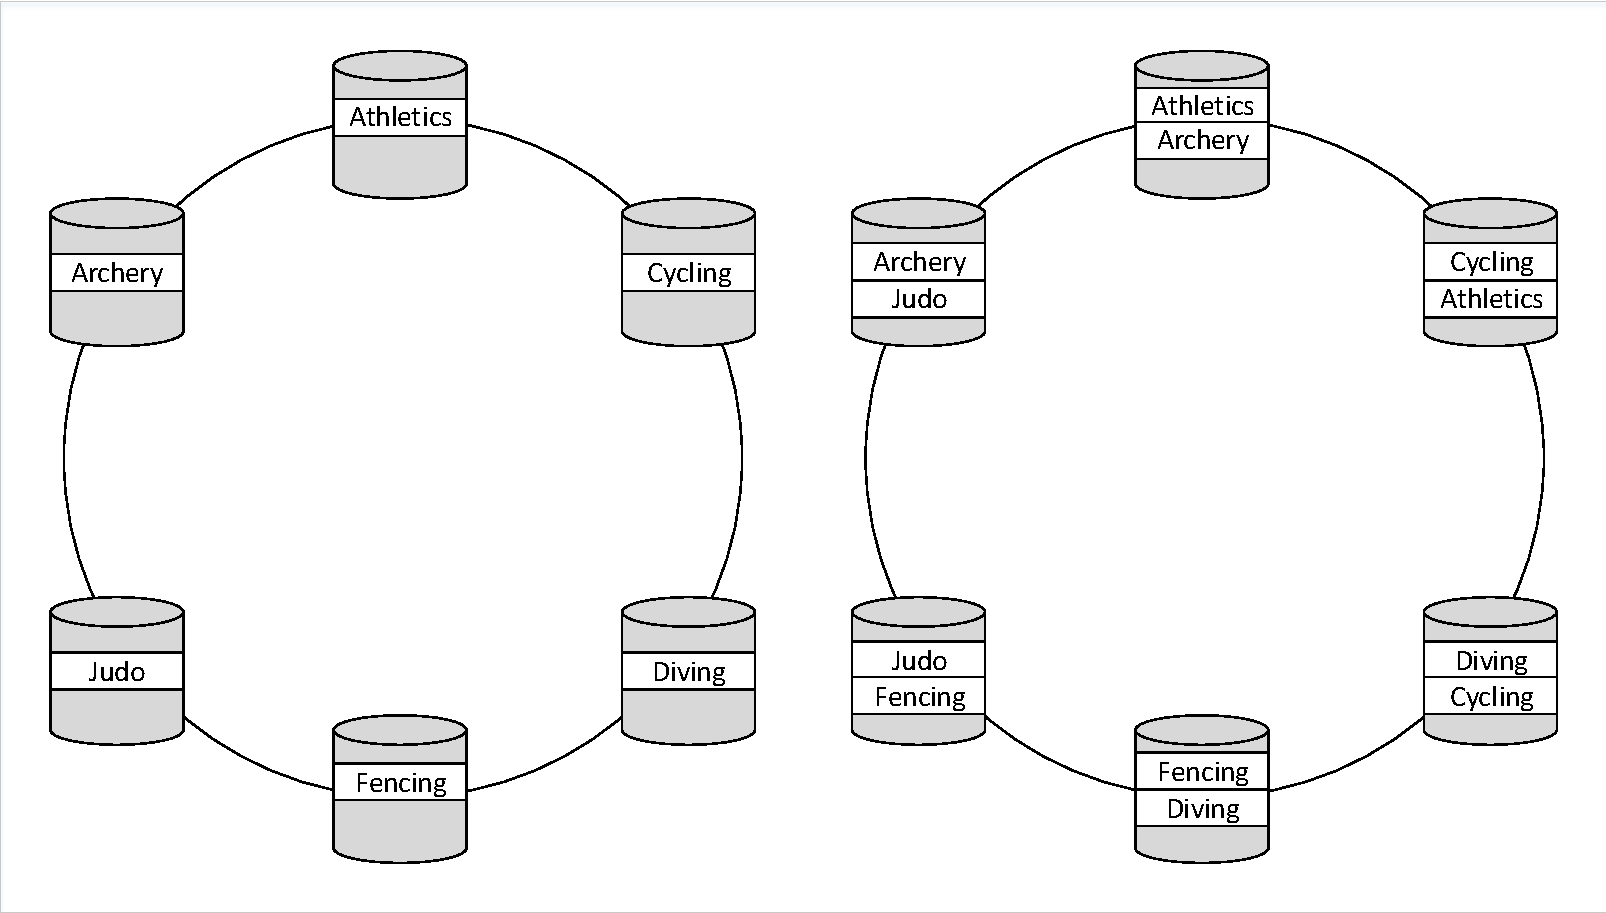
\includegraphics[trim = 5 5 5 5, clip, width=\textwidth]{img/dbdist}
\end{figure}
